\begin{frame}{Ultrasound hardware: another route into neurotech}
  \begin{columns}[c,onlytextwidth]
    \column{.55\textwidth}
      \small
      \NTXPoint{un0rick / pic0rick --- Luc Jonveaux}{Open pulse-echo hardware for learning, prototyping, and non-destructive testing.}
      \NTXPoint{Open-LIFU --- Openwater}{An open focused-ultrasound research platform: electronics, mechanical designs, firmware, planning, and simulation.}
      \NTXPoint{A place for community contributions}{Documentation, simulation, signal processing, and bench validation. Imaging and stimulation are different tasks.}
    \column{.41\textwidth}
      \centering
      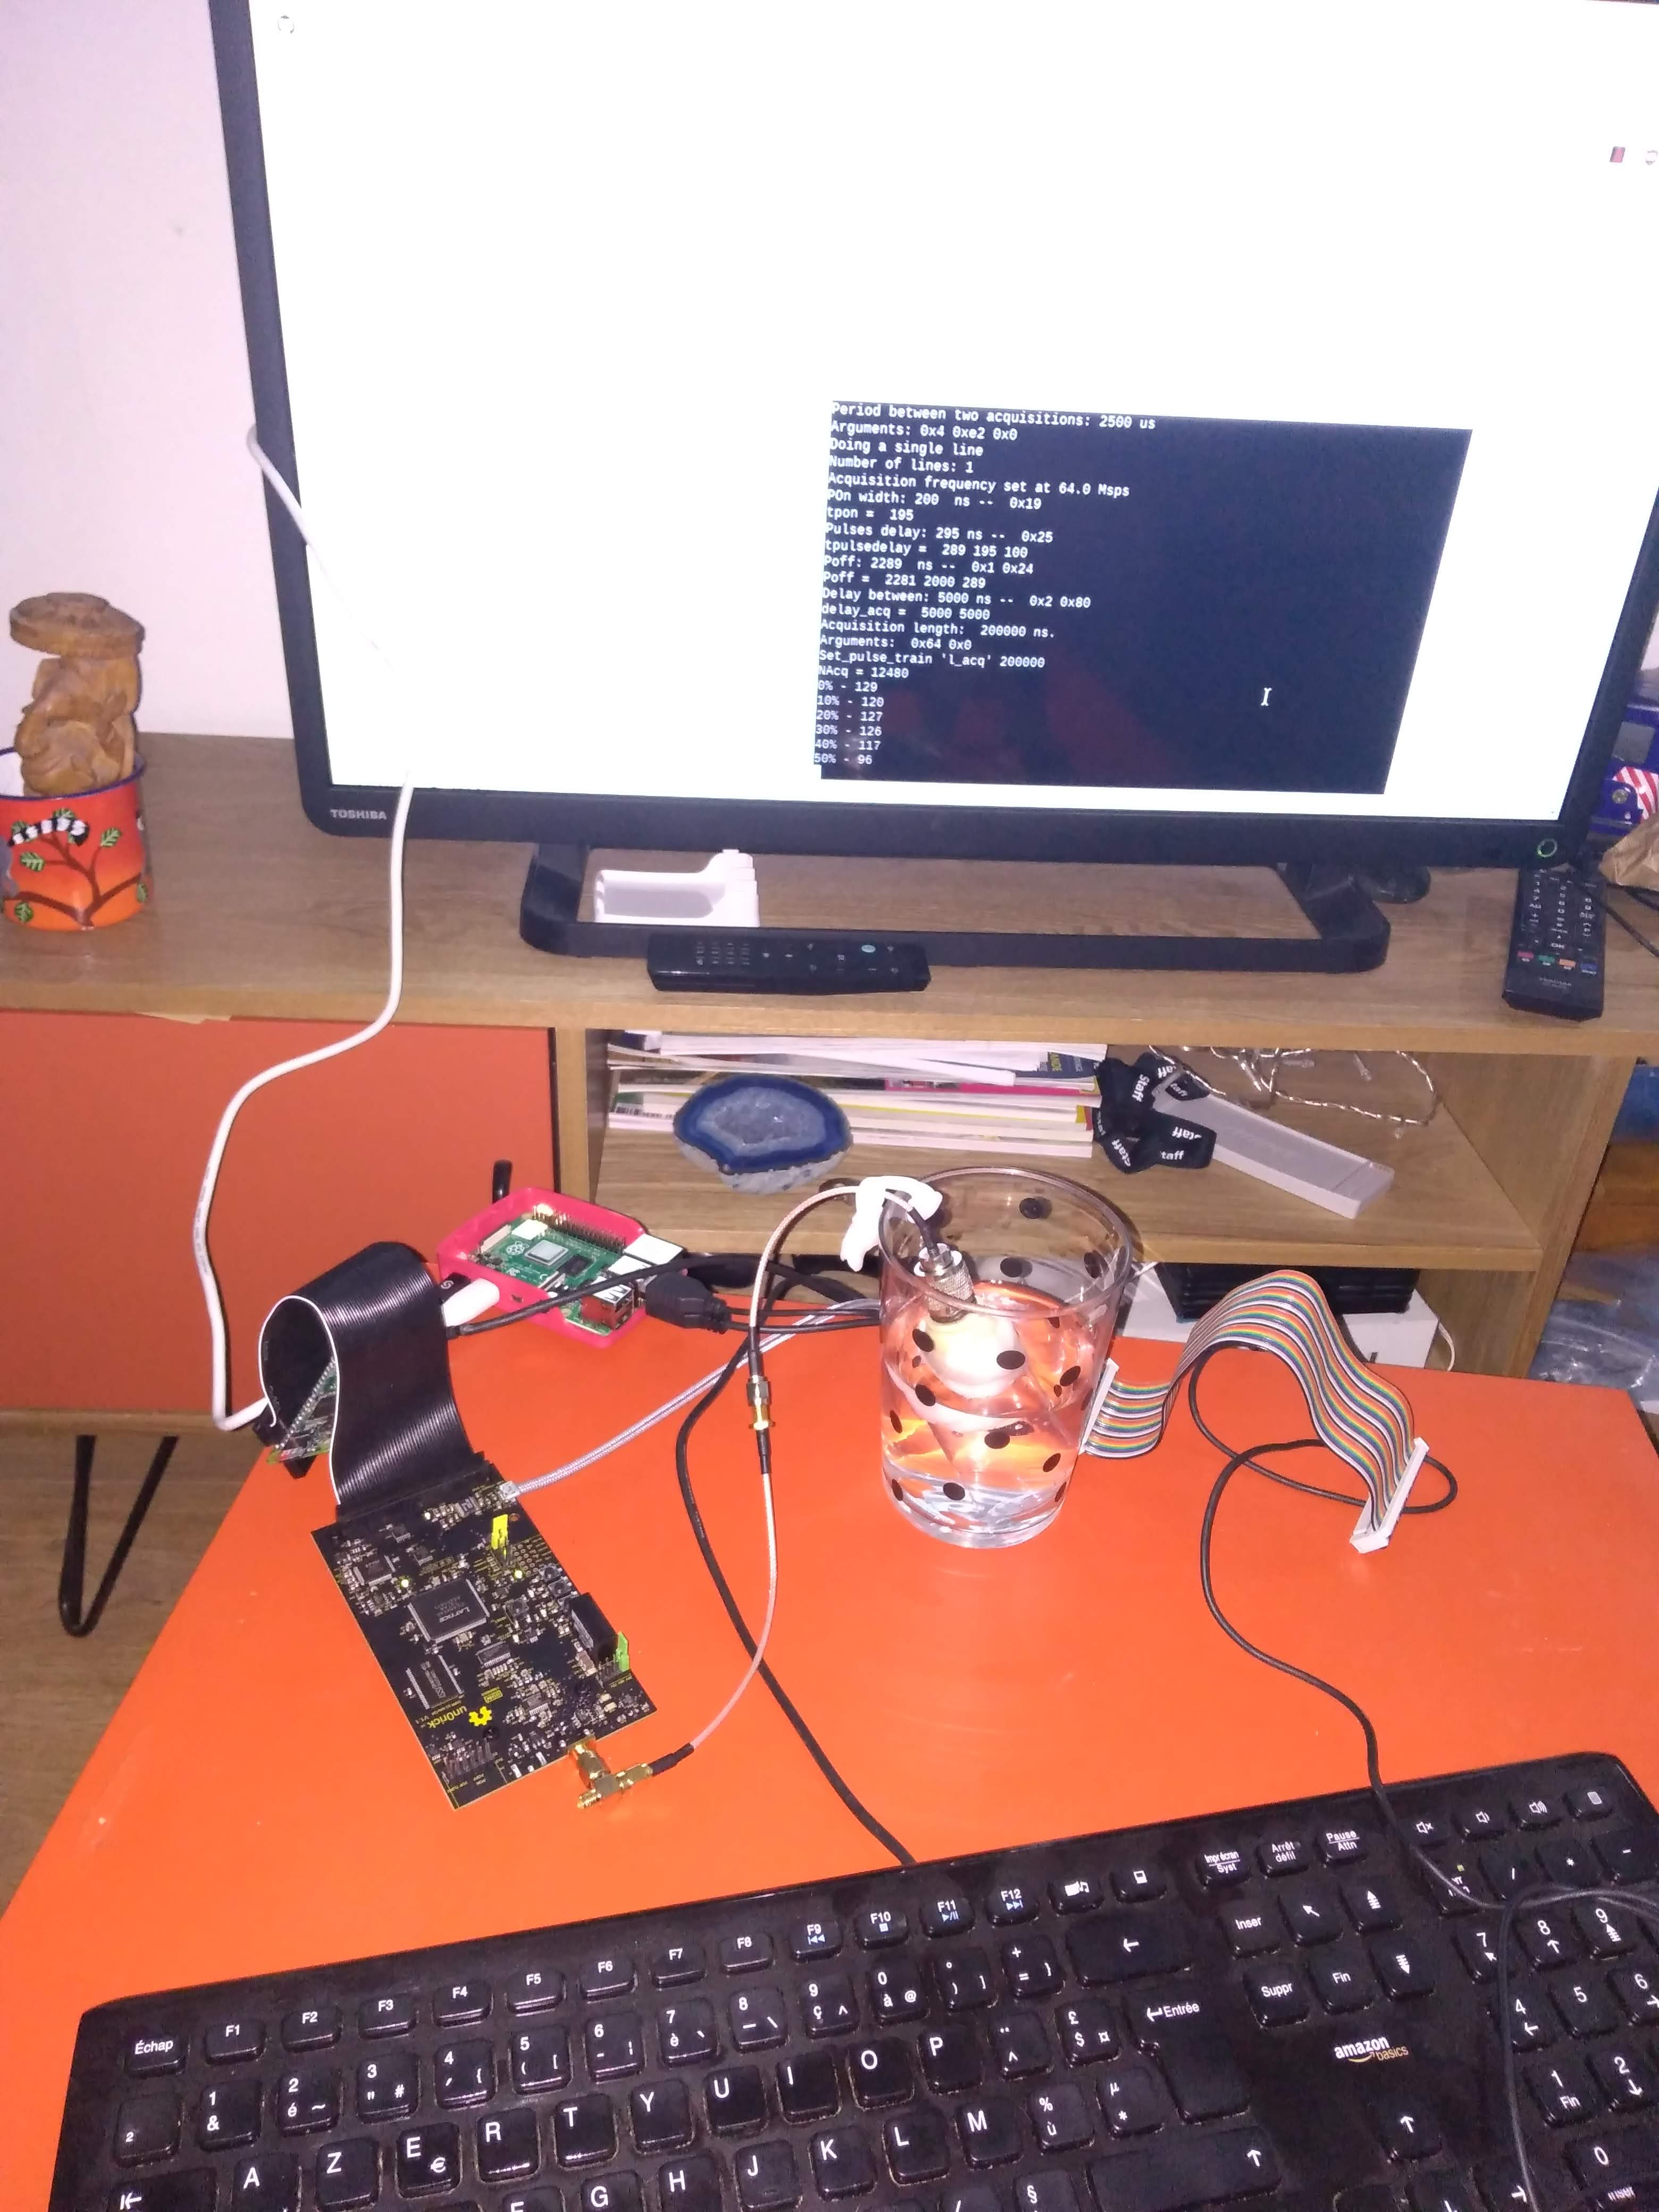
\includegraphics[width=\linewidth,height=43mm,keepaspectratio]{assets/history/un0rick-bench.jpg}\par\smallskip
      {\tiny Historical un0rick bench setup\newline Photo: Luc Jonveaux / kelu124, CC BY-SA 3.0\par}
  \end{columns}
  {\scriptsize Research hardware --- not a guide to self-administered brain stimulation.\par}
  {\tiny\color{NTXMuted}Sources: \href{https://un0rick.cc/}{un0rick open hardware}; \href{https://github.com/OpenwaterHealth}{Openwater platform repositories}\par}
  \note{[28:45--30:15] Expand the ultrasound example already introduced alongside OpenEIT. The un0rick lineage provides pulse-echo tools for learning and prototyping; the photograph shows a historical un0rick bench, not pic0rick or an Open-LIFU system. Openwater publishes separate focused-ultrasound research hardware and software repositories. Their inclusion illustrates available open research tools, not a claim that NTX owns, funds, or formally partners with either project. Do not imply that a pulse-echo board is interchangeable with a tFUS neuromodulation device or that low cost establishes diagnostic or clinical equivalence. Human stimulation requires appropriate research oversight, calibrated equipment, safety assessment, and qualified supervision. No operating parameters, human-use protocol, or claim of therapeutic efficacy is supplied. This leads into the local community that studies these methods together.}
\end{frame}

\begin{frame}{tFUS Society: a community around ultrasound}
  \begin{columns}[c,onlytextwidth]
    \column{.52\textwidth}
      \small
      \NTXPoint{Started with Leo Zaroff}{Bringing researchers, technical enthusiasts, and founders together around transcranial focused ultrasound.}
      \NTXPoint{Hosted by NeuroTechSF}{Meetings at Studio45/55 and Frontier Tower: talks, technical discussion, and shared projects.}
      \NTXPoint{From papers to shared work}{Project Sonus: ultrasound-imaging simulation and replication. Frontier Tower: a joint neuroimaging workshop with Lev Chizhov.}
    \column{.44\textwidth}
      \centering
      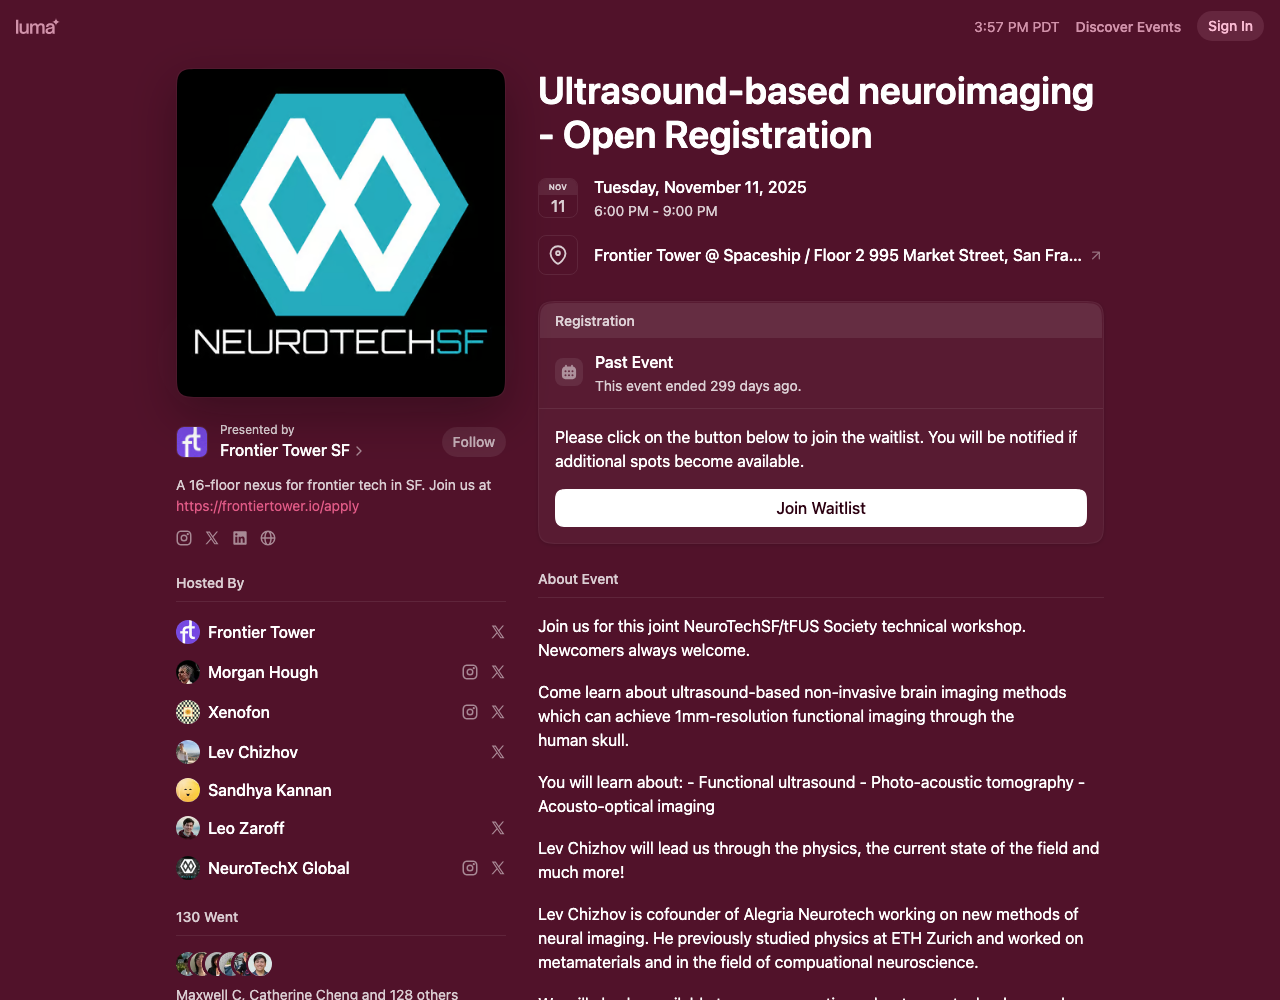
\includegraphics[width=\linewidth,height=46mm,keepaspectratio]{assets/history/tfus-frontier-event-page.png}\par\smallskip
      {\tiny Joint NeuroTechSF / tFUS Society workshop\newline Frontier Tower, November 11, 2025\newline Event-page screenshot --- not a meeting photograph\par}
  \end{columns}
  {\tiny\color{NTXMuted}Sources: \href{https://luma.com/e5kwzyvq}{Studio 55, November 6, 2024}; \href{https://luma.com/ultrasound-based-neuroimaging}{Frontier Tower workshop}; founding and Studio45 history: Morgan Hough\par}
  \note{[30:15--31:45] Morgan supplies the account that this was started with Leo and hosted by NeuroTechSF at Studio45/55 and Frontier Tower. Leo's public name is Leo Zaroff. His own April 2026 essay describes him as the founder of tFUS Society. Public Luma listings establish joint events and identify Morgan Hough, Leo Zaroff, and Nic Berry as hosts at the Studio 55 research-and-development meeting. Its local date is November 6, 2024 (UTC November 7). It describes Project Sonus as open-source simulation and replication of an academic full-waveform-inversion imaging paper; do not claim a completed working scanner or confuse imaging with stimulation. The November 11, 2025 Frontier Tower workshop lists Lev Chizhov and topics including functional ultrasound, photoacoustic tomography, and acousto-optical imaging. Its advertised resolution and safety claims are not independently adopted here. Studio 55 is verified in the public listing; Studio45 history is Morgan's supplied account, not an independently verified venue/date. RSVP labels are not audited attendance totals. No identifiable in-person meeting photo was located: the image is explicitly a screenshot of the actual event page. Replace it if Morgan supplies a verified event photograph.}
\end{frame}
